%--------------------------------------------------------%
  % Journal Article Manuscript Template

%% Copyright 2014 Nicholas E. Reith.
  
  % This work may be distributed and/or modified under the
  % conditions of the LaTeX Project Public License, 
  % either version 1.3 of this license or (at your option) 
  % any later version.
  
  % The latest version of this license is in
  %   http://www.latex-project.org/lppl.txt
  % and version 1.3 or later is part of all distributions of LaTeX
  % version 2005/12/01 or later.
  
  % This work has the LPPL maintenance status `unmaintained'.
  
  % This work consists of the files main.tex and subsidiary files:
  % (references: biblio.bib), (sections: content.tex, coverpage.tex,
  % preamble.tex, title_authors.tex, and title_noauthors.tex), and
  % (tables: sample_longtable.tex, and sample_table.tex).
  
  % It also includes the BibTeX reference styles: 
  % asr.bst, and ajs.bst, borrowed from here:
  % http://people.ku.edu/~chkim/

%--------------------------------------------------------%


%--------------------------------------------------------%
%	This is the main .tex file, which controls and combines
%	the other sections.
%	See the "sections" folder to edit content
%--------------------------------------------------------%

% GENERAL MANUSCRIPT TEMPLATE

	% by Nicholas E. Reith

	% DATE: November 26th, 2014

%--------------------------------------------------------%
%	PREAMBLE
%--------------------------------------------------------%

% DOCUMENT CLASS
    % Change "letterpaper" to "a4" if you use a4 paper size
    \documentclass[letterpaper,12pt]{article}
  
% TITLE SECTION
	
 %Abstract
    \usepackage{abstract} % Allows abstract customization
    % Set the "Abstract" text to bold
    \renewcommand{\abstractnamefont}{\normalfont\bfseries}
    % Set the abstract itself to small italic text
    \renewcommand{\abstracttextfont}{\normalfont\small\itshape} 

 %Title
    \usepackage{titlesec} % Allows customization of titles

 %Authors
    \usepackage{authblk} % For multiple authors

 %Date
	\usepackage{datetime} % allows for including today's date
  	% These two lines creates a new date format ``Month day(th), year''
    \newdateformat{usvardate}{
  	\monthname[\THEMONTH] \ordinal{DAY}, \THEYEAR}

% HEADERS & FOOTERS

 %Footnotes
  	\usepackage[bottom]{footmisc} % Makes footnotes stick to bottom of the page
    
 %Endnotes
	% Uncomment this line if using endnotes "\endnote{}"
	% \usepackage{endnotes}
    
 %Headers from page 2 on
    \usepackage{fancyhdr}
    \pagestyle{fancy}
    \fancyheadoffset{0cm}
    \setlength{\headheight}{15pt} 
 
% DRAFT WATERMARK
	% NOTE: Comment out these two lines to remove watermark
    \usepackage[firstpage]{draftwatermark} % adds draft watermark
    \SetWatermarkLightness{0.85}

% MACROS
    % Define keywords macro command
    \providecommand{\keywords}[1]{\textbf{\textit{Keywords---}} #1}

%% LianTze 7 Dec 2016:
%% Updated how the wordcount is implemented
\newcommand\wordcount{%
  \immediate\write18{texcount -utf8 -merge -sum -incbib -dir -sub=none -brief \jobname.tex | cut -d : -f 1 > 'count.txt'}%
  \input{count.txt}\ignorespaces words%
}
  

% MATH SUPPORT
    % The amssymb package provides various useful mathematical symbols
    \usepackage{amssymb}
    % The amsthm package provides extended theorem environments
    \usepackage{amsthm}
    % The newtxmath package provides additional math symbol support
    	% in Times New Roman symbols, etc.
    \usepackage{newtxmath}

% FONTS
    \usepackage{microtype} % Slightly tweak font spacing for aesthetics
    \usepackage[utf8]{inputenc}
    \usepackage{newtxtext} % Makes default font Adobe Times New Roman
  
% LINES
	% Spacing
	\usepackage{setspace} % See \doublespacing command at the top of content.tex
    % Numbering
    \usepackage{lineno,xcolor} 	% See \linenumbers at the top of content.tex

% MARGINS
	%NOTE: All spaces in this template are in inches, because it is
    % formatted for letterpaper (8.5 x 11 inch) paper. If you use a4
    % paper, choose different sizes in millimeters or centimeters.
	\usepackage[top=1.5in, bottom=1.5in, left=1in, right=1in]{geometry}

% COMMENTS
	\usepackage[colorinlistoftodos]{todonotes} % allows margin comments
    % See examples in content.tex, and here for manual: 
    % http://www.ctan.org/pkg/todonotes
	\usepackage{soul} % allows for highlighting
    
% GRAPHICS
    \usepackage{graphicx} % More advanced figure inclusion
    \usepackage{float} % For specifying table/figure locations, i.e. [ht!]
    
    % The printlen command allows the user to print the exact text width or height.
    % This is useful, when trying to create graphics (outside of LaTeX, of course)
    % with the optimal dimensions. See here for usage: http://www.ctan.org/pkg/printlen
    \usepackage{printlen}

% TABLES
    \usepackage{longtable} % For long tables that span multiple pages
    \newcommand{\sym}[1]{\rlap{#1}}% For symbols like *** in tables
    \usepackage{tabularx} % Allows advanced table features
    \newcolumntype{L}[1]{>{\raggedright\arraybackslash}p{#1}}
    \newcolumntype{C}[1]{>{\centering\arraybackslash}p{#1}}
    \newcolumntype{R}[1]{>{\raggedleft\arraybackslash}p{#1}}
    \usepackage{relsize} % Allows precise adjustment of font size,
    	%useful for fitting tables to page width

% REFERENCES
	\usepackage{hyperref} % For hyperlinks in the PDF

      % NOTE: This document uses bibtex for references
      % because both style files for Sociology Journals are
      % only available in .bst format. You can change to
      % biblatex if you prefer below.

      % Many thanks to Sociology Professor, 
      % ChangHwan Kim at the University of Kansas. 
      % for providing these .bst files here: 
      % http://people.ku.edu/~chkim
      
	% BIBTEX
    % Comment out this line if using biblatex
    \usepackage{chicago} % AJS and ASR styles rely on chicago

    % BIBLATEX
    % NOTE: Uncomment out these three lines to use biblatex
    % Be sure to put the biblio.bib file in biblatex format'
    %\usepackage{csquotes}
	%\usepackage[style=authoryear,backend=biber]{biblatex}
	%\bibliography{biblio}
    
 % See preamble.tex to edit the overall layout

% Header from Page Three on: Edit below for left and right headers
\lhead{}
\rhead{Inferring the temperature at which the Last Universal Common Ancestor lived}

%--------------------------------------------------------%
%	BEGIN DOCUMENT
%--------------------------------------------------------%

\begin{document}

%TC:ignore   %% This region is ignored for the word count
% COVER PAGE

%--------------------------------------------------------%
%	COVER PAGE
%--------------------------------------------------------%

\begin{titlepage}

  \newcommand{\HRule}{\rule{\linewidth}{0.5mm}} % Defines a new command for the horizontal lines, change thickness here

  \center % Center everything on the page


%	HEADING SECTION

  %\textsc{\LARGE University Name}\\[1.5cm] % Name of your university/college
  \textsc{\Large Thesis}\\[0.5cm] % Major heading such as course name
  \textsc{\large MSc Palaeobiology}\\[0.5cm] % Minor heading such as course title

%	TITLE SECTION

  \vspace{1.5 cm}
  \HRule \\[0.4cm]
  { \huge \bfseries Inferring the temperature at which the Last Universal Common Ancestor lived
}\\[0.4cm] % Title of your document
  \HRule \\[1.5cm]
 
%	AUTHOR SECTION

  
  \vspace{.5 cm}
  \large{\textsc{Edmund R. R. Moody}\\}
  \vspace{3 cm}
  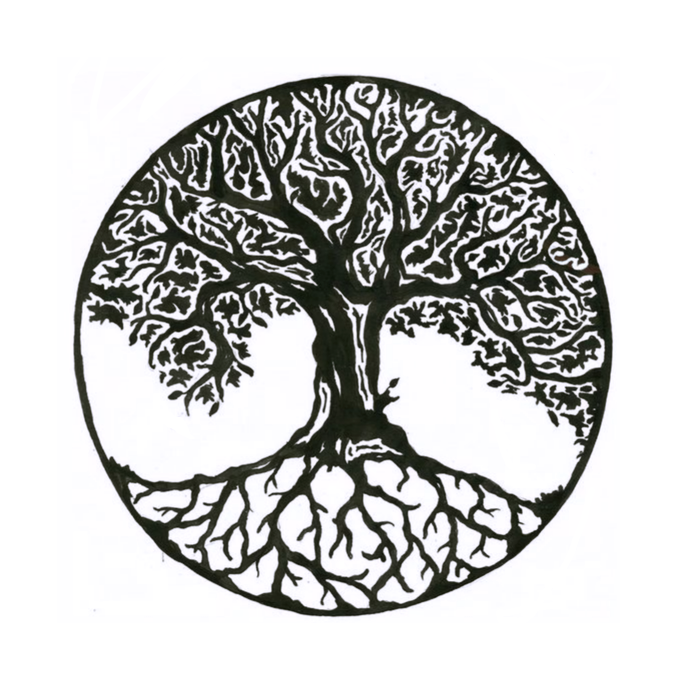
\includegraphics[width=0.25\textwidth]{figures/Treeoflife.png}
   \vspace{1 cm}
  
  
  Em16077@bristol.ac.uk\\
  Department of Earth Sciences,\\
  University of Bristol\\
  \vspace{.5 cm}

%	DATE SECTION




\vfill % Fill the rest of the page with whitespace

\end{titlepage}

%-----------------------------------------------------------------

\newpage % Comment out to remove cover page
%TC:endignore

\thispagestyle{empty} % Removes header on page two. Only needed if there is a coverpage

% TITLE SECTION

% Comment out one of the two lines below to include or exclude authors in article title. You may want to exclude them in case of a double-blind peer review submission, since authors appear on the cover page, and reviewers should not see the authors' names in the manuscript draft.

%%--------------------------------------------------------%
%	TITLE SECTION with authors
%--------------------------------------------------------%

% Article title
  \title{\vspace{-15mm}\fontsize{21pt}{10pt}\selectfont\textbf{Wordy Manuscript Title: \\Even Wordier Manuscript Subtitle\thanks{Draft manuscript. Please do not cite without the authors' permission.}}}

% Authors and Affiliations
  \author[1]{\large First Author}
  \author[1]{\large Second Author}
  \author[2]{\large Third Author}
  \affil[1]{\normalsize Department of XYZ, The University of ABC}
  \affil[2]{\normalsize Department of ABC, The University of XYZ}
  \renewcommand\Authands{ and }

% Today's date
	\date{Submitted: \usvardate\today}
%-----------------------------------------------------------
%	TITLE SECTION - with authors
%-----------------------------------------------------------

% Article title
  \title{\vspace{-15mm}\fontsize{21pt}{10pt}\selectfont\textbf{Wordy Manuscript Title: \\Even Wordier Manuscript Subtitle\thanks{Draft manuscript. Please do not cite without the authors' permission.}}}

% Today's date
	\date{Submitted: \usvardate\today}

\makeatletter
\renewcommand{\@maketitle}{
\newpage
 \null
 \vskip 2em%
 \begin{center}%
  {\LARGE \@title \par}%
 \end{center}%
 \par} \makeatother


\maketitle % Insert title

% NOTE: Comment out the lines below to remove line numbers
  % Running line numbers:
  %\linenumbers
  %\setlength\linenumbersep{15pt}
  %\renewcommand\linenumberfont{\normalfont\footnotesize\sffamily\color{gray}}
  %\pagewiselinenumbers % Same, but that reset on every page:
  %\modulolinenumbers[1] % Number only every line. Change for fewer.

%--------------------------------------------------------%
%	CONTENT
%--------------------------------------------------------%

% See the content.tex file for the abstract and body text


%--------------------------------------------------------%
%	ABSTRACT
%--------------------------------------------------------%

% NOTE: AJS Wants about 100 words.
%Abstract: Not exceeding 300 words; should be a comprehensive summary of your conclusions - a distillation of your thesis (i.e. a concise description of the problem(s) addressed, method(s) of solving them, and results). The abstract does not contain references. Write this after you have completed the report.

\begin{abstract}
\noindent Cellular life is split into domains, which share a Last Universal Common
Ancestor (LUCA). Understanding LUCA’s optimal growth temperature can help to elucidate the type of environment in which early life evolved. Here, we show that amino acid content can be used as an indicator for the optimal growth temperature of prokaryotes, even when only a small subset of the proteome is known. Amino acid compositions of extant organisms were examined for a group of specific amino acids, which were used to predict their growth temperature. These predictions were compared against reported values from the scientific literature and a strong correlation was found. We then reconstruct a proteome for LUCA, using a new phylogenetic model which improves upon the standard model. We conclude LUCA was a non-hyperthermophile; furthermore, we suggest that LUCA may have been a psychrophile. 




%To complete
\end{abstract}
\keywords{LUCA, Extremophile, Phylogenetics, Evolution, Microbiology, Proteome}
\newpage
\section{Acknowledgements}

Tom Williams most of all, for without him none of this would be even remotely possible, from helping with the technological aspects of the research to the more abstract concepts necessary for understanding, and of course having the idea for the project in the first place. Celine Petitjean who taught me some much needed bash at various crucial points during the project. Davide Pisani for teaching me phylogenetics and sparking my keen interest in the subject, as well as providing access to the data. Charles Deeks, whose keen eyes helped immensely. Bill Martin and Madeline Weiss, who provided us with the alignment data.

\section{Competing Interests}
We have no competing interests
 	
\section{Data, code and materials}
Data, code and materials are available on the University of Bristol Palaeobiology archive.

%update
\newpage
\section{Declaration}

"I declare that the work contained in this thesis is the author's own, except where stated or referenced. The views expressed in this thesis are those of the author and do not represent those of the University of Bristol."

 
%then signed by you and dated.\\

% Insert keywords here
\setlength\parindent{.45in} 

\newpage
\tableofcontents
\newpage
%--------------------------------------------------------%
%	BODY TEXT
%--------------------------------------------------------%

% Start double spacing here if you want
\doublespacing

% Main Text
\section{Introduction}
%Introduction: Introduction should be interesting. The first paragraph or two should be less dry than the scientific norm. Introduction should include what topic was addressed, and why it is important. Specimens, evolutionary problem, geological setting, etc. - a brief outline only; followed by a clear statement of the aims of your work in the final paragraph - "The aims of this project are to…".(Introduction starts on page 1 - previous pages in roman numerals). 
Darwin was one of the earliest to publish on the idea of the existence of a universal common ancestor in the Origin of Species: "Therefore I should infer from analogy that probably all the organic beings which have ever lived on this Earth have descended from one primordial form, into which life was first breathed"\cite{darwin1880origin}.

There is substantial evidence that all extant life on Earth shares a common ancestor. Some of the most compelling evidence for this includes the commonality of DNA triplet codons for the same identical 20 amino acids, and the chirality of the amino acids themselves (all amino acids coded for by DNA are the same enantiomer). This evidence is present across the domains: Bacteria, Archaea and Eukaryota. The means by which biological information is stored and used: DNA to RNA to protein synthesis is also conserved, as are the core mechanisms of transcription and translation via polymerases and \gls{ribosomes}. Further evidence is the common use of membrane proton gradients for energy via adenosine triphosphate (ATP) synthases. These similarities, as well as the comparative genetic evidence for the preservation of a genetic code pre-dating a common ancestor \cite{Knight2001} (figure 1), strongly support the relatedness of all life. Furthermore, molecular phylogenetics demonstrates that extant life is monophyletic \cite{Theobald2010}.

\begin{figure}
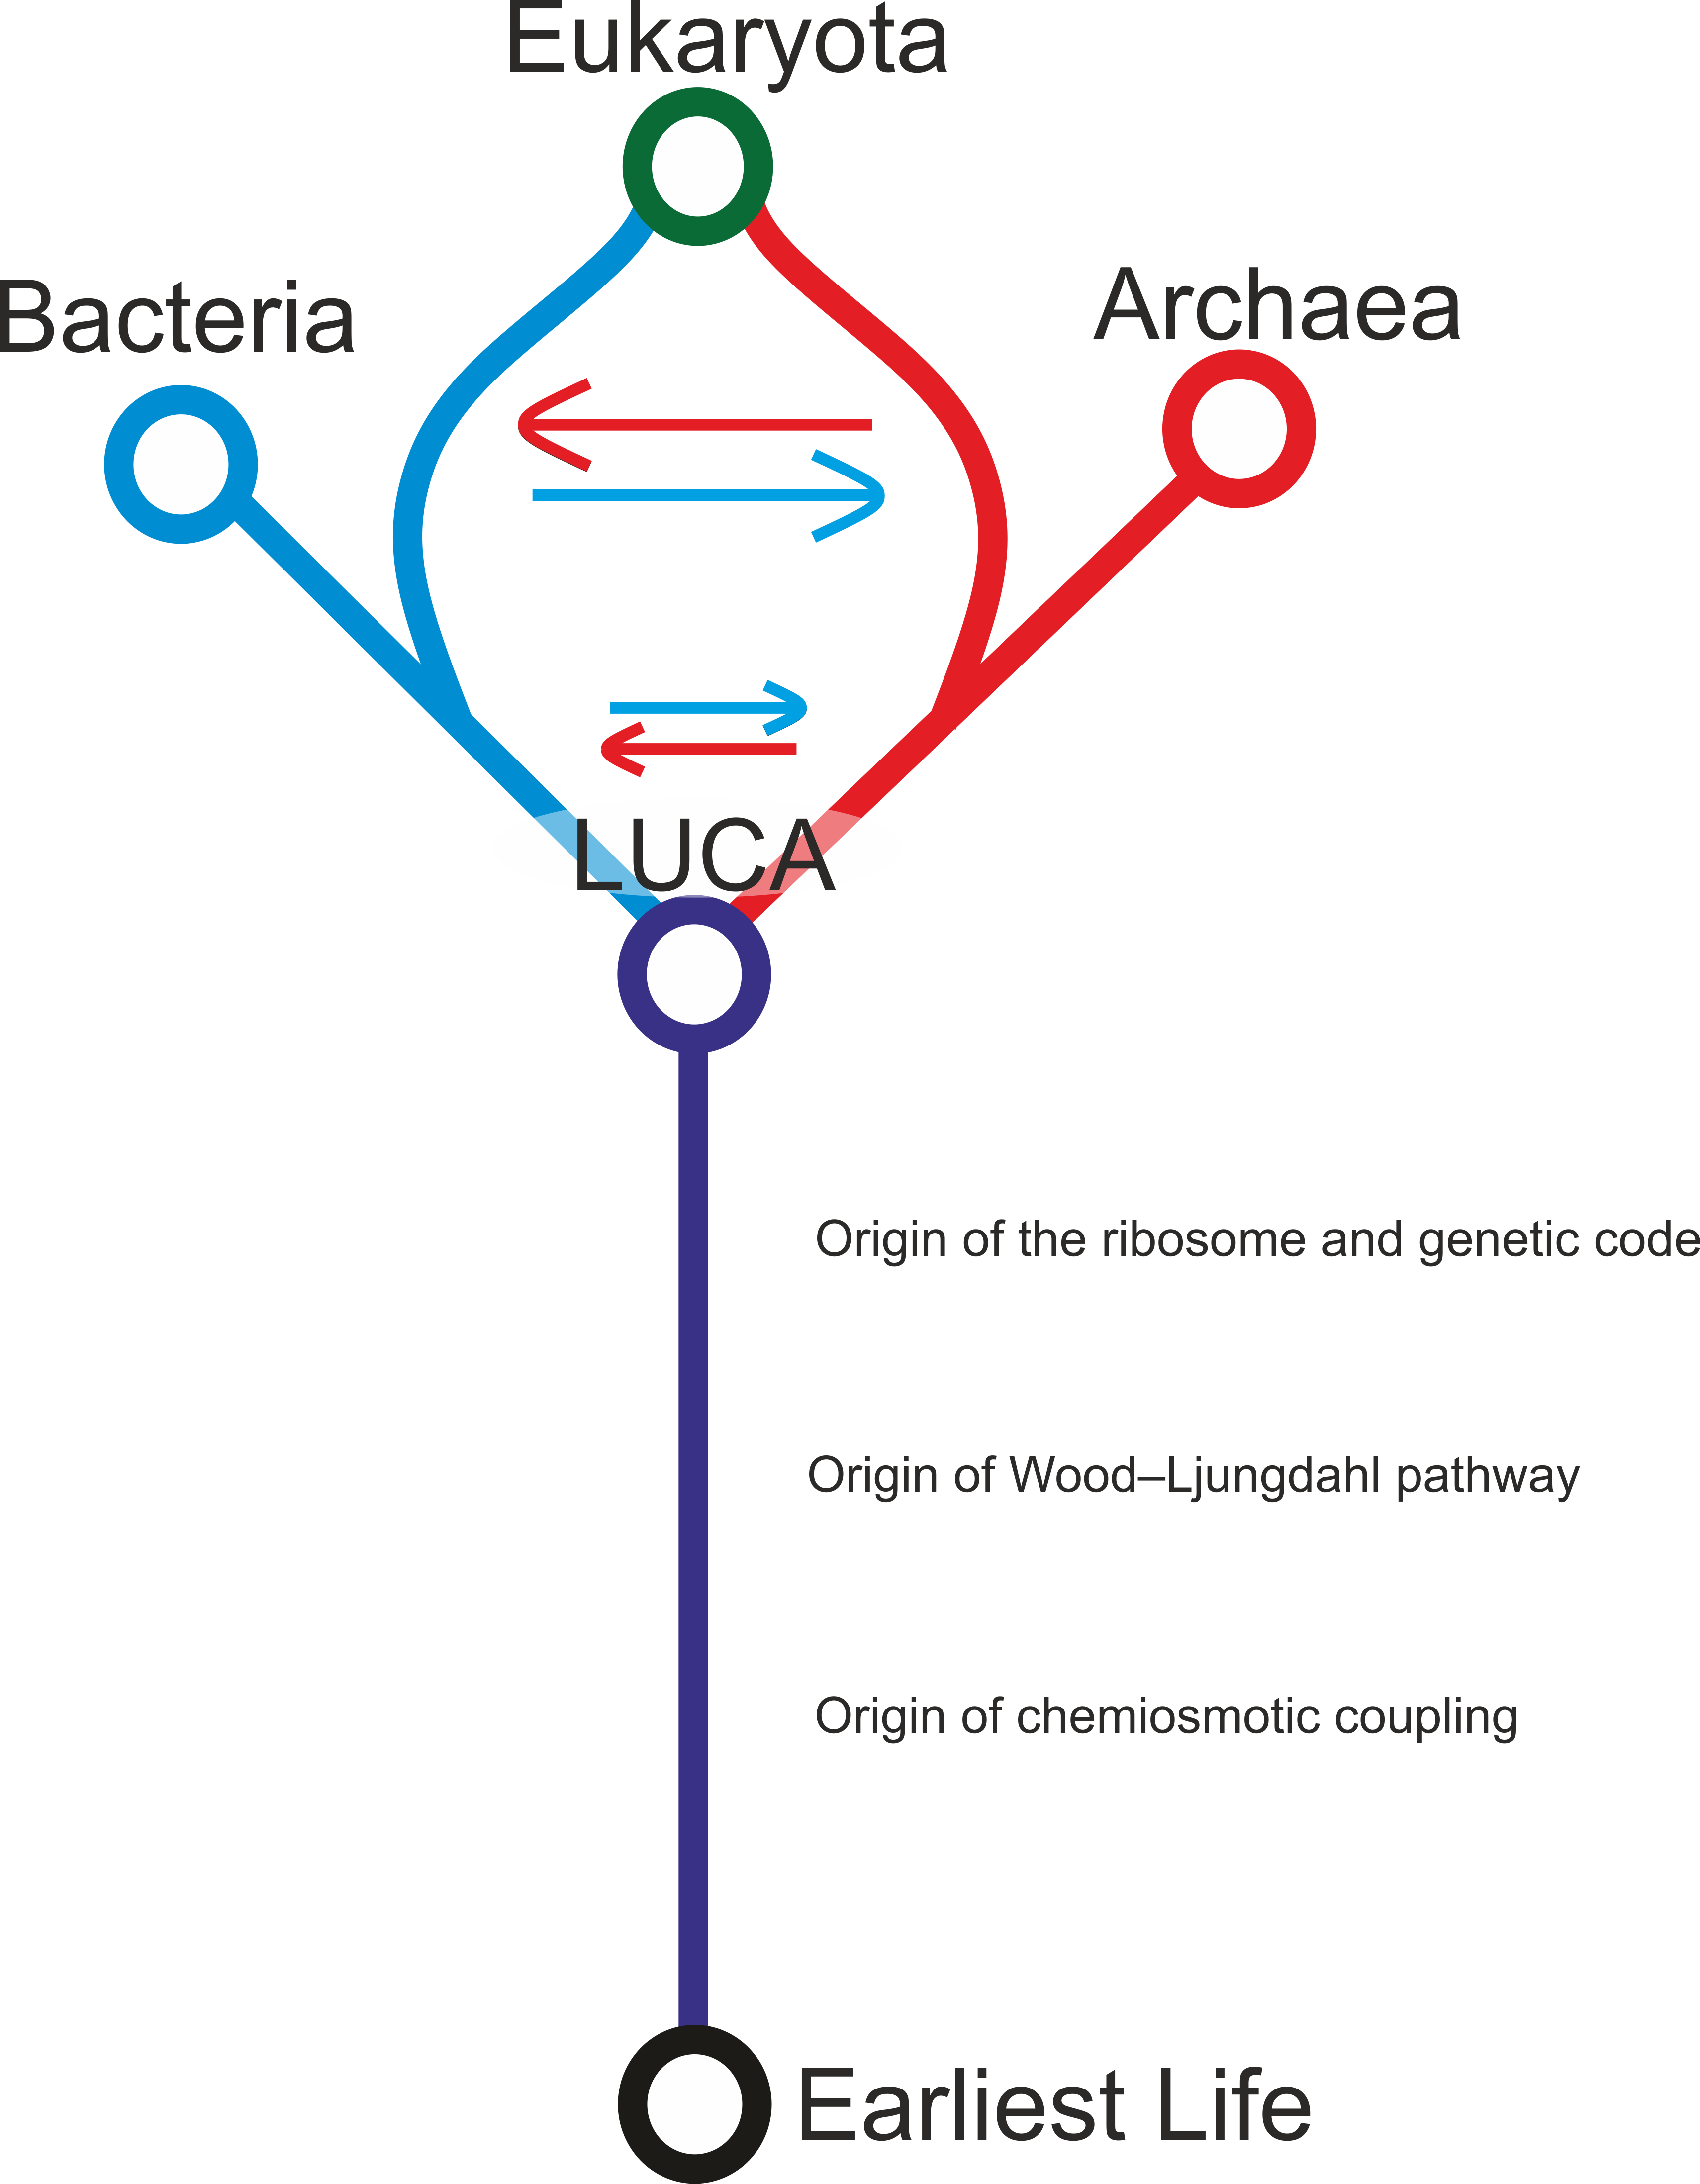
\includegraphics[width=0.7\textwidth]{figures/LUCATREE2.png}
\centering
\caption{\textbf{The context of LUCA within the tree of life.} Eukaryotes may have arisen from a symbiosis event between archaea and bacteria, therefore LUCA was the most recent common ancestor of Bacteria and Archaea. This diagram illustrates that LUCA was not necessarily the earliest life, and key adaptations such as the use of chemiosmotic coupling, the Wood-Ljungdal pathway \cite{weiss2016} and the genetic code itself are likely to have evolved before LUCA. The blue and red arrows represent the possibility of inter-domain lateral gene transfer taking place, which could cause complications when making phylogenetic inferences about LUCA from extant organisms.}
\end{figure}

Phylogenetic analysis of 16s ribosomal proteins suggests that all extant life falls into one of three domains: Archaea, Bacteria and Eukaryota \cite{woese1990towards,fox1977classification,garrett2014backward}. Recent work suggests eukaryotes were formed in a symbiosis of archaea and bacteria \cite{koonin2014dispersed}. Therefore, the last universal common ancestor (\gls{LUCA}) is the common ancestor of Archaea and Bacteria (figure 1). The question arises: what kind of organism was LUCA, and what type of environment did it inhabit?

Life can be categorised by the temperature at which the greatest growth occurs. These provide general definitions for describing different organisms into broad bands: hyperthermophiles possess an optimal growth temperature (\gls{OGT}) of $\geq$60°C, thermophiles possess an OGT between 50°C and 122°C, mesophiles are between 20°C and 45°C, psychrotrophs will survive at 0°C (but have a preference for more moderate temperatures), and psychrophiles grow optimally between -15°C and 10°C.

Studies based on nucleotide base pair frequencies show that it is likely that the earliest branches within the bacterial and archaeal domains were hyperthermophilic \cite{stetter2006hyperthermophiles}. However, there is still considerable debate as to whether LUCA itself was a hyperthermophile \cite{weiss2016,gogarten2016luca,boussau2008parallel,di2003universal}.

One line of evidence into LUCA's ecological preferences is through using genetic material as a `molecular thermometer' \cite{groussin2013molecular}. Double stranded DNA molecules contain paired nucleotides \cite{watson1953molecular}, the guanine and cytosine (GC) pairings share three hydrogen bonds, whilst adenine and thymine pairs (AT) have two. As a result, the proportion of GC:AT base pairs affects the melting temperature of duplex DNA, as more energy is required to break this higher number of hydrogen bonds \cite{vinogradov1971hydrogen}.

One approach is to use a phylogenetic model to infer GC content, but there is debate as to whether this correlates strongly with OGT. A strong correlation between the GC content of structural RNA and transfer RNA, rather than genomic DNA, with growth temperature has been reported \cite{hurst2001high,galtier1997relationships}. However, recent work suggests that nucleotide base stacking interactions are more important indicators of DNA thermostability \cite{yakovchuk2006base}.

%GC content figure
A non-hyperthermophilic LUCA was proposed based on ribosomal RNA sequence evolution \cite{galtier1999nonhyperthermophilic} and recently this has been supported by GC content inferred for LUCA \cite{boussau2008parallel}, in contrast to the hyperthermophilic ecology inferred for the last bacterial common ancestor and the archaeal common ancestor \cite{groussin2013molecular}. These compositions were modelled using a maximum likelihood phylogenetic analysis, assuming a branch-heterogeneous model of protein evolution \cite{groussin2013branch}. 

As an alternative to modelling GC content, some workers have drawn inferences about LUCA through a reconstruction of its gene content \cite{weiss2016}. A hyperthermophilic nature for LUCA was inferred based on shared genetic material across the bacterial and archaeal domains, although it has been suggested that this reconstruction could be subject to some bias due to lateral gene transfer (\gls{lgt}) \cite{gogarten2016luca} (figure 1).

In this study, we inferred the OGT of LUCA using a different approach. A general relationship between amino acid composition and OGT has long been established for modern prokaryotes \cite{saunders2003mechanisms,kreil2001identification} and recently this relationship has been described \cite{zeldovich2007}. First, we show that this relationship holds when analysing the subset of modern genes that can be traced back to LUCA \cite{weiss2016}. Then, we infer the ancestral amino acid \gls{compositions} of these gene products in LUCA using Maximum Likelihood (ML) under a non-stationary model, which allows for compositions to vary over time. Finally, we use these compositions to infer sequences for LUCA, the Last Bacterial Common Ancestor (\gls{LBCA}) and the Last Archaeal Common Ancestor (\gls{LACA}). Our results suggest that LUCA was a psychrophile in contrast to the hyperthermophilic LBCA and LACA \cite{schwartzman2004hyperthermophilic}. The ecology of LUCA will help us understand the possible environments early life may have evolved in, and may help us understand the limits of where life could arise elsewhere in the universe.

\section{Materials and methods}

%Materials and methods: Analytical approaches, field techniques, data handling methods. It should be possible to reproduce exactly what you have done. Also list repositories of material and terminology.
 
\subsection{Inferring sequences and alignments}

We obtained the alignment data used in this study from Weiss \textit{et al.} \cite{weiss2016}. This comprised of 355 alignment files that were generated using a ML tree reconstruction on proteins from 1,981 extant species (134 archaea and 1,847 bacteria). These alignments were the only ones to preserve domain monophyly and were found in both Bacteria and Archaea. 

We inferred ML trees using the LG \cite{le2008improved}, LG + C60 \cite{si2008empirical} and LG + PMSF models \cite{wang2017modeling}. In all three models we use a discrete gamma model to account for rate heterogeneity across sites within sequences \cite{yang1994maximum}. In this study we use four rate categories to approximate the distribution, with equal probability for each category \cite{yang1994maximum}. Empirical amino acid frequencies were counted from our alignment data and we used bootstraps (1000 replications) to assess the reliability of our phylogenetic trees  \cite{soltis2003applying}.

The first phylogenetic model we use is the Le and Guascel (LG) general amino acid replacement matrix \cite{le2008improved}. This model allows for the variability of evolutionary rates across sites in the matrix estimation in addition to the maximum likelihood estimation which assigns probabilities to phylogenetic trees by inferring a probability distribution from standard statistical techniques. 

%DISCUSSION This model was by far the most efficient time wise and in terms of computing power needed, but also produced the fewest number of monophyletic trees (with respect to the two domains).

We have also used a protein mixture model, the C60 model \cite{si2008empirical}, which accounts for site-specific amino acid replacement patterns. The C60 model configuration possesses 60 components of the protein mixture model. This variant was chosen as it produces more robust phylogenetic reconstructions at the expense of greater required computing power \cite{si2008empirical}. In our reconstruction, C60 is used a variant of the CAT model (named as it classifies sites into categories), which assumes the existence of distinct classes for amino acid replacement patterns at different sites of a protein alignment to be described by a distinction substitution process \cite{lartillot2004bayesian}. These are both used for a maximum likelihood reconstruction. A Poisson distribution amino acid replacement, with equal amino acid exchange rates and frequencies was assumed, as well as gamma rate heterogeneity among sites.

We used the PMSF (posterior mean site frequency) model as a rapid approximation for a small number of trees. The PMSF are the amino acid profiles for each alignment computed from an input mixture model and a guide tree. Our guide trees were created using the LG model (above). The PMSF model was chosen for its speed and its ability to improve long branch attraction artefacts\cite{wang2017modeling}.

\subsection{Zeldovich's method}
Zeldovich \textit{et al.} \cite{zeldovich2007} established that OGT highly correlates with the amino acid composition of proteomes in prokaryotes. Seven amino acids: isoleucine, valine, tyrosine, tryptophan, arginine, glutamic acid and leucine, have been determined as the best predictors of OGT \cite{zeldovich2007}. A linear relationship has been derived using a linear regression between the proportion of these seven amino acids in the \gls{proteome} and the observed OGT for 86 bacterial species \cite{zeldovich2007}. The relationship between the ratios of these amino acids and the OGT was given as:

\[T_{opt} = 937F -355\]

\noindent where $T_{opt}$ is the optimal growth temperature of an organism in \textdegree C, and \textit{F} is the fraction of the seven specific amino acids in the entire proteome \cite{zeldovich2007}. This relationship was used in our study to predict the OGT of our reconstructed LUCA sequences.

In order to determine the accuracy and reliability of this relationship when using a subset of the proteome, experimental OGTs from extant organisms were tested against our equation-inferred predictions. The species and protein sequences chosen for our predictions were based on the protein sequence alignments originally collected by Weiss \textit{et al}. These proteins were inferred as the gene products which can be mapped back to LUCA \cite{weiss2016}. The experimental OGT data were obtained from the scientific literature and two databases: BacDive \cite{sohngen2013bacdive} and the NCBI \cite{o2015reference}. We used linear regression, implemented in Matplotlib \cite{hunter2007matplotlib}, to evaluate the relationship between composition of sequences and OGT for the species used in our analysis. Due to time constraints and limited resources, a small representative sub-sample of extant species was used (n=208) for this assessment of the accuracy of Zeldovich's equation.

\subsection{Utilizing the alignment data}

To determine the reliability of Zeldovich’s equation using only the test set of protein sequence alignments (above), the alignment files were analysed in Python (figure 2) using the Biopython module \cite{chapman2000biopython}. The fraction of the seven indicative amino acids was calculated for each separate protein sequence within each devised alignment using a further Python module, NumPy \cite{walt2011numpy}, to produce a predicted OGT using Zeldovich’s equation \cite{zeldovich2007}. These predictions were collated to produce an OGT specific to each species. For the 1,981 species, a different inferred temperature was calculated for each species and gene alignment. In order to link each local gene identifier (used by Weiss \textit{et al.}) in the alignment files to their respective species in the taxonomy list, an associative array was created using the Python module, Pandas \cite{mckinney2010data}.

\begin{figure}
\includegraphics[width=0.4\textwidth]{figures/Codediagram.png}
\centering
\caption{\textbf{A flow diagram describing the Python script we wrote to infer optimal growth temperature from alignments.}}
\end{figure}

%figure of python script flow chart

%Bio++ libraries were used \cite{gueguen2013bio++}.

%\subsection{Analysing the amino acid content of specific proteins}
%As Reverse gyrase  is indicative of hyperthermophilic organisms \cite{forterre2002hot,atomi2004reverse}. We test the amino acid composition of reverse gyrase, using Zeldovich's equation \cite{zeldovich2007} to predict an optimal growth temperature. The sequence for reverse gyrase was taken from the hyperthermophilic bacterium \textit{Pyrobaculum calidifontis} obtained from UniProt \cite{uniprot2014uniprot} (UniProt identifier: A3MU01-1).


\subsection{Rerooting the phylogenetic trees}
A Python script was written to reroot the maximum likelihood trees, inferred by the above models, at the split between Archaea and Bacteria. The trees that could not be rerooted were rejected as they were not found to preserve domain monophyly. 

%DISCUSSION Even though previous research using this data \cite{weiss2016} suggests that all the alignments generate monophyletic after maximum likelihood inferred trees, this was found not to be the case with the models used here (see discussion).

\subsection{Two new non-homogeneous models}
We used the phylogenetic tool-kit p4 \cite{foster2004modeling}, in order to construct our own models allowing for a non-homogeneous composition across trees. This allowed us to have a different composition for the root of the tree (LUCA) compared to the rest of the tree. This produced a Maximum Likelihood ancestral state reconstructions from a non-stationary distribution. Our first model infers the ancestral amino acid sequences for LUCA based on the inferred trees by setting one composition at the root of the tree and one elsewhere, using LG exchangeability.
In order to simplify the calculations, our second model uses binary data which we generated from recoding our protein sequence alignments. In our second model we set five compositions: one each for LUCA, LBCA, LACA, the \gls{crown group} of Archaea and the crown group of Bacteria.

%figure of non-stationary distribution on a graph

\section{Results and Discussion}

\subsection{Estimating optimal growth temperatures for the sequence composition of ancient genes}

In order to verify whether the relationship between amino acid composition and OGT is consistent when using only the set of 355 genes that Weiss \textit{et al.} \cite{weiss2016} could map back to LUCA.  We wrote a Python script (figure 2) \cite{chapman2000biopython} to calculate the values for Zeldovich's equation \cite{zeldovich2007} for the sequence alignments of extant species.

As there were 1,981 species, we opted to use a small sub-sample (n=208). The predicted values for OGT were then compared to the reported OGT values. The correlation co-efficient (r) was 0.906, showing a strong correlation between these two variables. The mean absolute error between the predicted and experimental values was 7.0°C, the median absolute error was 5.0°C and the modal error was 2.0°C. At the extremes, the least accurate predictions were 30°C above and 22°C below reported. 

The equation works more reliably as a predictor at higher temperatures ($\geq$40°C), as when comparing organisms with an OGT of <40°C, we find a much weaker correlation (r=0.344). This trend continues with a slightly higher average deviation at lower temperatures (5.0°C) compared to the average deviation for predictions higher than 40°C which was (4.6°C). In order to observe whether or not this was a result of bias in the protein sequence alignments we analysed the entire set of alignments. Our results show that the majority of the extant organisms used in the dataset are mesophilic and there were many instances of the same species being used multiple times. The majority of the species present in the alignment data also possessed an OGT of 37°C. To adjust for this, we removed the values for organisms with a reported OGT of 37°C and observed the new correlation (figure 3). This then showed a stronger correlation (r=0.940). The mean predicted OGT for the entire sub-sample was 45°C, whereas the overall mean for the experimental values was only 4°C away at 41°C. The standard deviation for the difference between predicted and experimental OGT was 6.2°C.

\begin{figure}
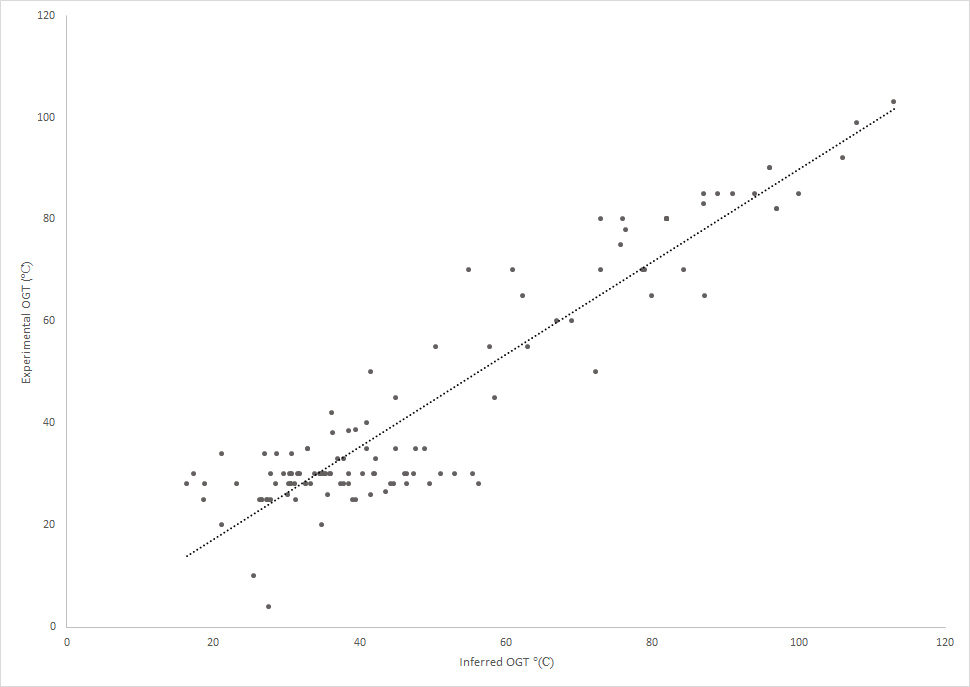
\includegraphics[width=\textwidth]{figures/experimental.png}
\centering
\caption{\textbf{This is the relationship between our inferred optimal growth temperatures (OGT) against the experimental OGT.} This graph shows the strong correlation between our OGT values inferred through using Zeldovich's \cite{zeldovich2007} equation and the reported OGT for the organism. The graph here shows the trend when we remove the reported 37°C values. The correlation r=0.940 is shown in this graph, indicating a very strong correlation, when including the reported 37°C values, we observe a correlation r=0.906.}
\end{figure}

This study evaluates the reliability and accuracy of using amino acid composition as an indicator of temperature adaptation in prokaryotes, specifically when using subsets of protein amino acid sequences. It appears that specific trends in amino acid usage show temperature adaptation in prokaryotes, without accounting for the organism's genomic GC content and regardless of its taxonomic position. These findings firmly support the notion of convergent evolution at the level of proteome composition with regards to adaptation \cite{johns2004evolutionary}, particularly to high temperature environments \cite{reed2013protein}. Our results show that Zeldovich’s \cite{zeldovich2007} estimate of OGT, which was inferred from whole proteome data, also works on the subset of genes that can be mapped back to LUCA.

An empirical correlation between the OGT of prokaryotes and the melting point of its proteins has been firmly established over the last three decades, \cite{vina2002biochemical,mcfall1990comparative,gromiha1999important} and it has been shown that specific amino acids can be used as a determinant of thermal adaptation \cite{zeldovich2007} and thermostability of proteins in thermophiles \cite{nakashima2003compositional,fukuchi2001protein}. Amino acid composition is not the only important indicator of temperature - details of hydrophobic interactions and surfaces charges have been shown to perform a key role in determining a protein's thermostability \cite{saelensminde2009amino}, as well as significant temperature-dependent differences between core and surface amino acid residue distributions \cite{saelensminde2007structure}. There appear to be marked differences between different ecological niches, with psychrophiles and mesophiles sharing similarities in their composition compared to that of thermophiles \cite{saelensminde2007structure}. Macromolecular adaptation to extreme environments has also been linked in other cases, such as halophilic (salt-loving) organisms, with specific proteome composition, characterized by Asp, Val, Thr and lower usage of Cys \cite{paul2008molecular}. These adaptations were found to be present irrespective of genomic GC-content and taxonomic position; if such mechanisms can be generalised, then this only further reinforces the importance of this study. Previous work has been mainly concerned with complete proteomic data or structural interactions between amino acids. This study will test, for the first time, this relationship when only a subset of the proteome is available.

Although the absolute mean error for our sub-sample was only 7.0°C and there is a strong correlation between the predicted and experimental OGT, there are limitations, with a maximum over-prediction of +30°C and a maximum under-prediction of -22°C. Predictions made on the borders between the descriptive groups could potentially result in the wrong classification. However, in the majority of cases, the error is minimal, and using these predictions serves as a broad indication of ecological temperature classification rather than an exact estimate.

As only a small sub-sample was used in the interests of time, a large sample or different sampling technique could produce different results. This said, as our predictions are highly accurate, this is unlikely. At higher temperatures (>40°C), a better correlation is found. One explanation for this could be that higher fractions of the seven specific amino acids may not distinguish as well between lower temperatures e.g. psychrophilic and mesophilic ecologies. This is consistent with results suggesting psychrophilic and mesophilic adaptations in amino acid composition are more similar to each other than to thermophiles \cite{saelensminde2007structure}. Data for mesophiles may be distorted as many are reported to have an OGT of 37°C. If these OGTs were taken experimentally, then this could indeed show a fault in the method. However, as 37°C is the OGT for many mammals this may be used as a default laboratory condition rather than being experimentally established.

The seven amino acids discussed here (Ile, Val, Tyr, Trp, Arg, Glu and Leu) are all attached to their cognate tRNA using class I aminoacyl-tRNA synthetases \cite{dutta2010analysis}. The preference for thermostability may be indicated in the translation mechanism rather than some intrinsic property of these residues within their proteins \cite{zeldovich2007}. Our results also suggest different usage levels of class I and class II synthetases during evolution, with more class I in LBCA and LACA (hyperthermophiles), than LUCA.

Our results show that Zeldovich's equation \cite{zeldovich2007} works well as a broad indication of an organism's OGT, but the prediction should not be taken as an exact reading. Nonetheless, it is still a useful and important result and this study suggests another way to learn about extinct organisms when only limited data are available. 


\subsection{Reconstructing the sequences and OGT of LUCA}

To reconstruct the sequences of each of the 355 genes present in LUCA, we first inferred phylogenetic trees using a maximum likelihood tree reconstruction. Only 226 trees were produced which retained domain monophyly (out of a possible 355 trees). Then, based on evidence for ancient gene duplications \cite{iwabe1989evolutionary,gogarten1989evolution} we wrote a Python script to reroot the trees between Archaea and Bacteria (129 of the inferred trees were not monophyletic and as such were rejected). From this, we inferred ancestral sequences at the root of the tree (corresponding to LUCA) using P4 \cite{foster2004modeling} in our two compositions model, and for LUCA, the root of Bacteria, the root of Archaea, crown group Archaea and crown group Bacteria in our five compositions model. 

We wrote Python scripts in order to infer OGT from the reconstructed amino acid sequences for LUCA from both our models. The OGT predictions for these reconstructed sequences vary greatly (figure 4). In the two compositions model, the highest prediction was 175°C and the lowest was -114°C. Both the mean and median OGT predictions place LUCA as a thermophile at 49°C and 56°C respectively. The majority of the predictions lie between 50°C and 75°C, which also places LUCA in the thermophile group. These results display a normal distribution with the highest number of OGT predictions between 75°C and 50°C, with the predictions for higher and lower respective OGT being even fewer in both directions.

However, in our five compositions model, the highest prediction was 283°C, and the lowest was -197°C. The mean OGT was 25°C, the median OGT prediction was 26°C. The majority of the predictions lie below 20°C, placing LUCA in the psychrophile group. The results from this set of data also display a normal distribution but the highest number of OGT predictions are between mesophilic to psychrophilic levels. 

The extreme variation in the per-gene estimates is expected, and is probably due to gene-specific compositional requirements (e.g. each gene has a different function, and perhaps some functions need to make use of more of a particular type of amino acid). On a single gene basis, effects like this could cause variation around the "average" composition for a particular OGT.

From this analysis, we can safely conclude that LUCA was not a hyperthermophile; but why do we see such a higher temperature estimation from the two compositions model? A possible explanation is that in the two compositions model, the inferred composition of LUCA is being distorted by exceptionally high inferences of OGT for LBCA and LACA. In our five compositions model, both LBCA and LACA are predicted to have OGTs well above 200°C, making them extreme even for hyperthermophiles. As the five composition model is more representative, we suggest that LUCA was a psychrophile. 

The extremely high LBCA and LACA estimates may also indicate that the relationship between the specific amino acids (Ile, Val, Tyr, Trp, Arg, Glu and Leu) and OGT observed by Zeldovich \cite{zeldovich2007} for modern sequences may not hold through time. For example, early in life's history, the proportion of those amino acids might also have been influenced by the relative availability of class I and class II aminoacyl-tRNA synthetases, or of other amino acids. It is also possible that the coefficient in the equation might itself evolve through time, reflecting the evolving cell environment. 

\begin{figure}
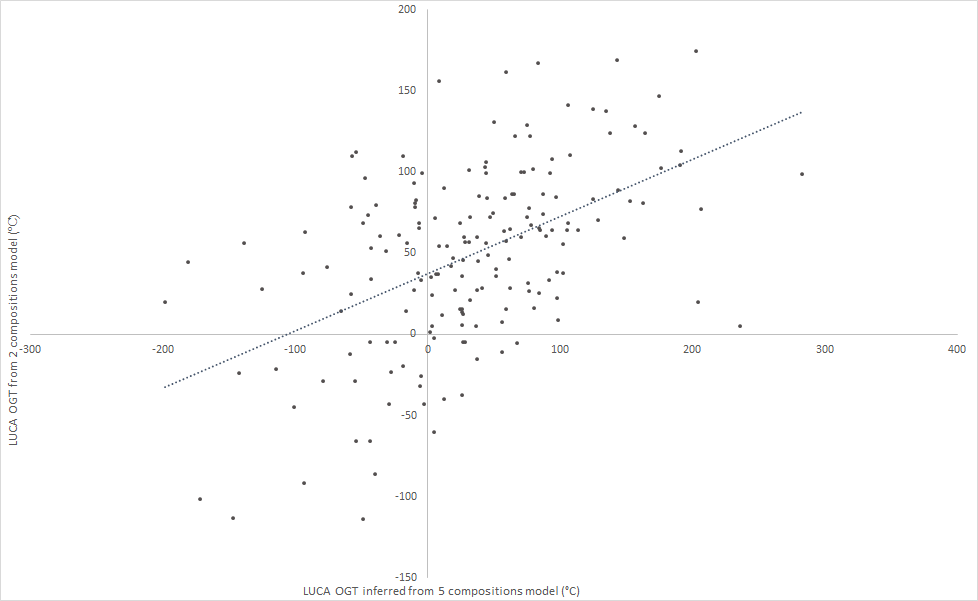
\includegraphics[width=\textwidth]{figures/compare.png}
\centering
\caption{\textbf{The relationship between the inferred LUCA optimal growth temperature from the five compositions model (y axis) against the inferred LUCA optimal growth temperature from the two compositions model (x axis).} Each point represents a protein within LUCA, this shows a positive correlation between the two models, albeit not a strong one (r=0.530).}
\end{figure}

The main purpose of this study was to determine whether an accurate OGT for LUCA could be predicted from reconstructed ancestral state amino acid sequences. Understanding LUCA, in any way, helps us consider how early life evolved and the way life has progressed. In order to understand biological evolution, we need to understand the history and the context of that evolution. 

We predict LUCA was not a hyperthermophile, with the majority of our five composition model's reconstructed sequences implying the OGT of LUCA was below 20°C. Darwin famously hypothesized that "in some warm little pond with all sorts of ammonia and phosphoric salts, light, heat, electricity etcetera present, that a protein compound was chemically formed" \cite{follmann2009darwin}. Our results show a cooler pond may be closer to the truth. It has been suggested that early life could have evolved in hydrothermal or volcanic systems \cite{mulkidjanian2012origin}, with an environment conducive for chemical reactions which also allows for natural light as an energy source \cite{mulkidjanian2012origin}. The chemical richness of these environments may be necessary for early RNA-like oligomers \cite{ricardo2004borate,grew2011borate}. Hydrothermal vents \cite{baross1985submarine} are chemically rich habitats where microbes flourish and there are similarities between the chemistry of hydrothermal systems and metabolic reactions in prokaryotic autotrophs \cite{martin2008hydrothermal,lane2010did}. 

There is also geological evidence for life in similar environments. Precipitates from seafloor-hydrothermal-vents have been interpreted as potential fossilised micro-organisms in sedimentary rocks \cite{dodd2017evidence}. This fossilized evidence can be dated to at least 3.7Ga and broadly agree with dates from biogenic carbon \cite{bell2015potentially}. These fossils push us closer to a date for early life and potential habitats consistent with our results for LBCA and LACA, suggesting a hyperthermophilic environment. Modern vents range in water emission temperatures from 30°C (diffuse vents) to over 400°C (black smokers), although there are local high temperature fluctuations down to lows of 2°C from the surrounding seawater \cite{lutz1993ecology,minic2006adaptation}. Amino acids can also be polymerised to peptides under geochemically relevant conditions (hydrothermal or volcanic systems) \cite{huber1998peptides}. 

Implications from rRNA based phylogenetic analyses \cite{woese1987bacterial,pace1997molecular} and GC content \cite{galtier1999nonhyperthermophilic} indicate that LUCA was not capable of withstanding higher temperatures, although this has been been subject to criticism \cite{di2003universal}. Inferring ancestral amino acid changes in 3-isopropylmalate dehydrogenase, Miyazaki \textit{et al.} reported that when introducing mutations extrapolated from ancestral amino acid sequences into the enzyme from an extant thermophile, the majority of the mutants showed a higher thermal stability than the wild-type, thus concluding LUCA to be a hyperthermophile \cite{miyazaki2001ancestral}. However, the elevation was marginal or negative in all these variants, suggesting the extrapolation was not robust. 

A psychrophilic LUCA is consistent with hypotheses regarding cooler earlier life, and there is chemical evidence suggesting a cold origin of life is possible \cite{miller1995origin}. One explanation is that proteins and RNAs originated at different times. One potential mechanism for molecular self-replication via RNA has been demonstrated through \textit{in vitro} evolution of a catalyst directly in cold water \cite{attwater2013ice} and a potential precursor to amino acids, hydrogen cyanide, has been shown to polymerize in greater concentrations at lower temperatures \cite{miyakawa2002cold}. Our results infer that the majority of the proteins present in LUCA were adapted to lower temperatures and may imply a cooler origin. Life may have arisen for the first time at any temperature, however a major impact or sudden environmental changes may have destroyed the majority of life on the early Earth, resulting in the psycrophilic LUCA we infer, already pre-adapted to survive the selection pressures \cite{schwartzman2004hyperthermophilic}.

Our results are consistent with the limits of the thermal stability of RNA \cite{martin2003origins}. As our prediction for LUCA's OGT is not hyperthermophilic, this is more favourable towards the stability and assembly of these primal organic molecules \cite{martin2003origins,moulton2000rna}.

Our results disagree with those of Weiss \textit{et al.} \cite{weiss2016}, who used ML to produce an estimate of genes that may have been present in LUCA, pointing to a hyperthermophilic LUCA, metabolically similar to extant methanogens. However, this research has been subject to criticism, as there is the possibility of false positives, due to LGT within orders \cite{gogarten2016luca}, and false negatives, as incomplete ATP synthases were inferred for LUCA when the complete enzyme would be required \cite{gogarten2016luca}.

\subsection{Our phylogenetic models}

Amino acid and nucleotide substitution models applied in phylogenetic analyses rely on simplified assumptions that the composition of amino acids or nucleotides has been identical through time, and that the evolutionary process has been reversible, stationary, homogeneous \cite{groussin2013branch} and without variation across different lineages \cite{groussin2013branch,jayaswal2011reducing}. Homologous sequences can vary widely in their amino acid or nucleotide base compositions \cite{zeldovich2007,dutheil2008non} meaning that sequence evolution rates have been altered amongst lineages. This is not accounted for by the standard models \cite{galtier1997relationships}. If composition is assumed to be the same across the entire phylogenetic tree then it follows that all branches possess the same rates of substitution, leading to incorrect phylogenetic hypotheses. A truly representative model would assume a different composition for every branch of the tree, although this would be computationally expensive. To address this, we use two non-homogeneous models (figure 5),  which assume that the composition of the root is different to those of the branches, sampling from a non-stationary distribution. One of our models (two compositions) simply assumes a different composition for the root (LUCA) compared to the rest of the tree, whereas the other assumes a different composition for LUCA, LBCA, LACA, crown group Bacteria and crown group Archaea. Thus our models are more representative of the evolutionary process than previous phylogenetic analyses. Our model uses ML, which has been implemented previously \cite{yang2000phylogenetic} for rate heterogeneity amongst sites in addition to process heterogeneity amongst lineages but originally such methods were limited by available computing power, limiting these methods to five sequences or less \cite{galtier1998inferring}.

\begin{figure}
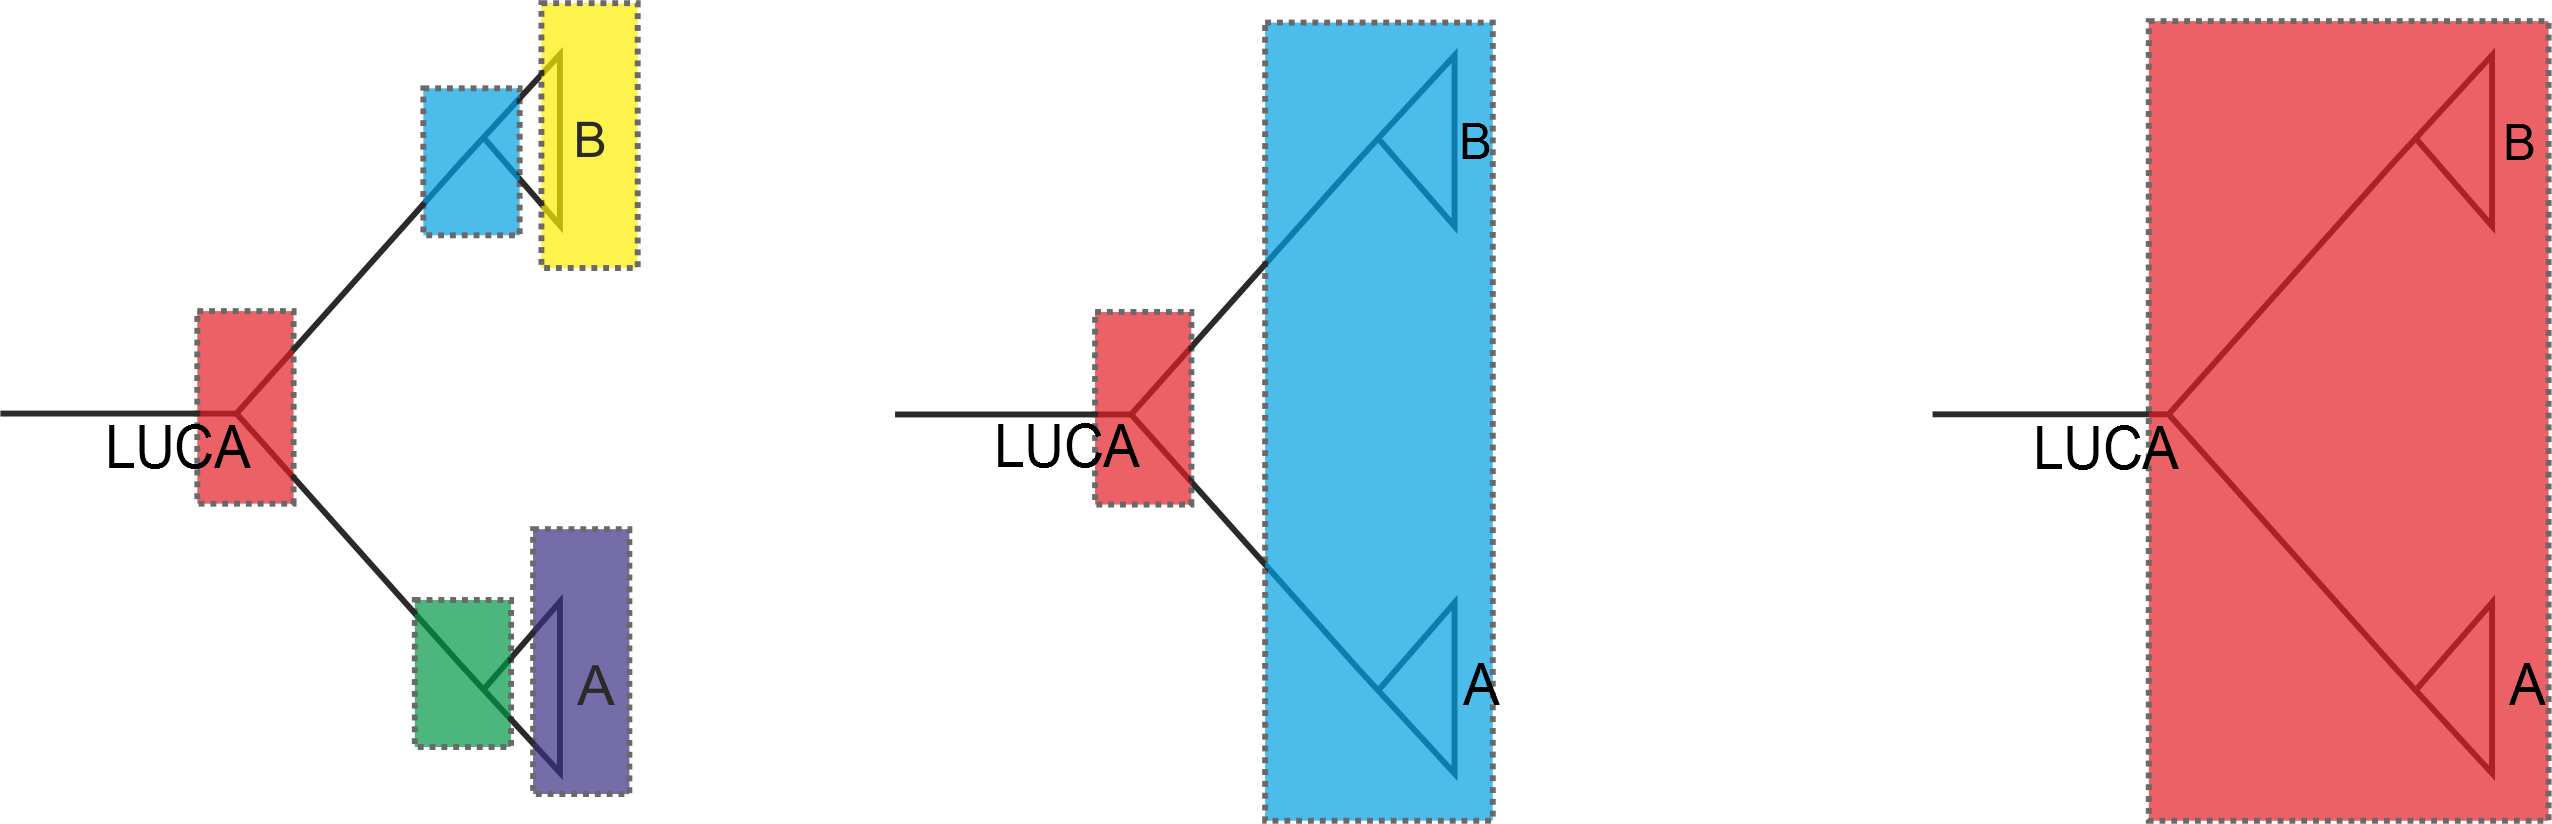
\includegraphics[width=\textwidth]{figures/modelcomparison3.png}
\centering
\caption{\textbf{A diagram illustrating how our five compositions model (left) and our two compositions model (middle) differ to the standard model (right).} The standard phylogenetic model (right) assumes the same composition all over the tree, whereas both our models (left and middle), set a variable composition. Our five compositions model (left) allows for a seperate composition at the root of the tree (LUCA), as well as at the root of both Bacteria (B) and Archaea (A), and at the crown group of both Bacteria and Archaea. Our two compositions model (middle) assumes a seperate composition for LUCA and for the rest of the tree, which are more representative than the current standard model (right), which does not allow for the differences.}
\end{figure}

Using the standard LG model \cite{le2008improved}, preserving archaeal and bacterial monophyly was not guaranteed. Only 226 out of possible 355 trees were monophyletic, which highlights a difference between the results of Weiss \textit{et al.} \cite{weiss2016} and those presented here. There are various possible explanations for this; one being that the LG model simply is not powerful enough to infer trees from the protein sequence alignments. As we used multiple models, and none of them returned all 355 trees, another explanation could be that the alignment data used are not monophyletic and are a result of multiple trans-domain gene transfer events \cite{gogarten2016luca}; if so, a re-evaluation of the dataset is recommended. 

\section{Conclusion}

\subsection{Overview and exploring implications}
Our study has explored the effectiveness of using amino acid composition of gene products as indicators of optimal growth temperature in prokaryotic organisms. We adopt an existing method, Zeldovich's equation, and use it in the context of phylogenetic ancestral state reconstruction. We conducted an experiment to test if, by examining the proportion of seven specific amino acids, we could predict optimal growth temperature from only limited sets of protein sequences (from a limited number of genes rather than the entire proteome of an organism). We compared our inferred predictions of OGT to reported OGTs from the literature. Our results have shown that amino acid composition works effectively as a general indicator of OGT. We applied this to reconstructed ancestral state sequences, in this case in LUCA. As these sequences are only generated from extant organisms, experimental data from extinct species is unobtainable. Therefore, such reconstructed sequences may never be wholly accurate, but the results of this study mean that we are closer to understanding the nature of organisms where only limited proteomic/genomic data are available.

Another application could be where only partial data are available, such as degraded or ancient sequences obtained from ice-cores or PCR amplified samples. Further examples of applications could be in regard to environmental DNA (eDNA) or metagenomic data. Although finding specific species in eDNA can be an arduous task, using these broad methods could help indicate the ecologies of the species involved.
The main focus of our study was to reconstruct amino acid sequences for LUCA. We used a ML phylogenetic analysis using a non-homogeneous model (allowing for a different composition for the root of the tree i.e. LUCA, and the rest of the tree). From this, we inferred a set of sequences for LUCA. Our results infer that LUCA would have been a psychrophile in contrast to LBCA and LACA (hyperthermophiles).

If LUCA was a psychrophile, then early life was adapted to colder temperatures. This supports the RNA world hypothesis, and could imply a colder origin of life. In contrast to this, the conclusion that LBCA and LACA are hyperthermophiles is consistent with geological evidence for the instability of the Earth's crust and climate at that time. The subsequent radiation of Bacteria and Archaea (and reduction of OGT in certain branches) could then be a result of the stabilisation of the later Earth's climate and establishment of the Earth's crust. 

\subsection{Final thoughts}

The topic of our earliest ancestors is interesting on a fundamental philosophical level. `Where did we come from?' is one of the most striking and prevalent questions we, as a species, have asked since we have possessed the ability to question the world. I hope this research helps us understand a small part of life's beginnings and our earliest ancestors. Nevertheless, there is still much more to be done.  Understanding LUCA is only the beginning; this work helps identify LUCA as a psychrophile but we need to seek a deeper understanding of the limiting factors.


 



%--------------------------------------------------------%
%	REFERENCE LIST
%--------------------------------------------------------%
\newpage
\singlespacing

% BIBTEX

    % NOTE: Comment out next two lines if using biblatex
%     \bibliographystyle{pnas2009.bst}
    \bibliographystyle{pnas-new-bare}
	\bibliography{references/biblio} % Insert bibliography
	
% BIBLATEX

	% NOTE: Uncomment next line to use biblatex
	% \printbibliography

%--------------------------------------------------------%
%	END NOTES
%--------------------------------------------------------%

	% Uncomment these three lines below if using endnotes
    % instead of footnotes
      % \newpage
      % \section*{End Notes}
      % \theendnotes

%--------------------------------------------------------%
%	FIGURES
%--------------------------------------------------------%

% NOTE: If your submission guidelines don't require figures
% at the end, you can comment out the two lines below,
% and embed figures in the text of content.tex instead of here

%\newpage
%\section*{Figures}

%\begin{figure}[ht!]
%\centering
\includegraphics[width=0.4\linewidth]{figures/placeholder}
%\caption{Figure caption}
%\end{figure}

%--------------------------------------------------------%
%	TABLES
%--------------------------------------------------------%

% NOTE: If your submission guidelines don't require tables
% at the end, you can comment out the two lines below,
% and embed tables in the text of content.tex instead of here

%\newpage
%\section*{Tables}

%%----------------------------------------------------------
%	TABLE: SAMPLE LONG TABLE
%----------------------------------------------------------

% NOTE: Both arrastretch and relscale below are set to 1.
% To expand or compress the table, change these to be larger
% or smaller than 1.

% Position, Spacing and Sizing
\begin{center}
\renewcommand*{\arraystretch}{1} % Set vertical stretch
{\relscale{1} % Set font size scale
% See other sample_table.tex for an example of using adjustbox
% to adjust the width of the table if necessary

% Begin Table and Caption
\begin{longtable}[H!]{@{\extracolsep{\fill}}lrrr}
\caption{Sample Table of Results} \\

% First header
\hline
\multicolumn{1}{c}{\textbf{Column 1}} & \multicolumn{1}{c}{\textbf{Column 2}} & \multicolumn{1}{c}{\textbf{Column 3}} & \multicolumn{1}{c}{\textbf{Column 4}} \\ \hline 
\endfirsthead

% Subsequent headers
\multicolumn{3}{c}{\tablename\ \thetable\ -- \textit{Continued from previous page}} \\
\hline
\multicolumn{1}{c}{\textbf{Column 1}} & \multicolumn{1}{c}{\textbf{Column 2}} & \multicolumn{1}{c}{\textbf{Column 3}} & \multicolumn{1}{c}{\textbf{Column 4}} \\ \hline 
\endhead

% First footer
\hline \multicolumn{3}{r}{\textit{Continued on next page}} \\
\endfoot

% Subsequent footers
\hline
\endlastfoot

% Meat of table

Row 1   & 0.1 & 0.5  & 10   \\
Row 2   & 0.2 & 1    & 20   \\
Row 3   & 0.3 & 1.5  & 30   \\
Row 4   & 0.4 & 2    & 40   \\
Row 5   & 0.5 & 2.5  & 50   \\
Row 6   & 0.6 & 3    & 60   \\
Row 7   & 0.7 & 3.5  & 70   \\
Row 8   & 0.8 & 4    & 80   \\
Row 9   & 0.9 & 4.5  & 90   \\
Row 10  & 1   & 5    & 100  \\
Row 11  & 1.1 & 5.5  & 110  \\
Row 12  & 1.2 & 6    & 120  \\
Row 13  & 1.3 & 6.5  & 130  \\
Row 14  & 1.4 & 7    & 140  \\
Row 15  & 1.5 & 7.5  & 150  \\
Row 16  & 1.6 & 8    & 160  \\
Row 17  & 1.7 & 8.5  & 170  \\
Row 18  & 1.8 & 9    & 180  \\
Row 19  & 1.9 & 9.5  & 190  \\
Row 20  & 2   & 10   & 200  \\
Row 21  & 2.1 & 10.5 & 210  \\
Row 22  & 2.2 & 11   & 220  \\
Row 23  & 2.3 & 11.5 & 230  \\
Row 24  & 2.4 & 12   & 240  \\
Row 25  & 2.5 & 12.5 & 250  \\
Row 26  & 2.6 & 13   & 260  \\
Row 27  & 2.7 & 13.5 & 270  \\
Row 28  & 2.8 & 14   & 280  \\
Row 29  & 2.9 & 14.5 & 290  \\
Row 30  & 3   & 15   & 300  \\
Row 31  & 3.1 & 15.5 & 310  \\
Row 32  & 3.2 & 16   & 320  \\
Row 33  & 3.3 & 16.5 & 330  \\
Row 34  & 3.4 & 17   & 340  \\
Row 35  & 3.5 & 17.5 & 350  \\
Row 36  & 3.6 & 18   & 360  \\
Row 37  & 3.7 & 18.5 & 370  \\
Row 38  & 3.8 & 19   & 380  \\
Row 39  & 3.9 & 19.5 & 390  \\
Row 40  & 4   & 20   & 400  \\
Row 41  & 4.1 & 20.5 & 410  \\
Row 42  & 4.2 & 21   & 420  \\
Row 43  & 4.3 & 21.5 & 430  \\
Row 44  & 4.4 & 22   & 440  \\
Row 45  & 4.5 & 22.5 & 450  \\
Row 46  & 4.6 & 23   & 460  \\
Row 47  & 4.7 & 23.5 & 470  \\
Row 48  & 4.8 & 24   & 480  \\
Row 49  & 4.9 & 24.5 & 490  \\
Row 50  & 5   & 25   & 500  \\

% End table and settings
\end{longtable}
}
\end{center}

%\newpage
%%----------------------------------------------------------
%	TABLE: SAMPLE SHORT TABLE
%----------------------------------------------------------

% NOTE: If you want to stretch or constrain a table
% to a particular width, such as textwidth, comment out
% the tabular code below, and uncomment the tabularx code.
% Using the "X" option, only available in tabularx allows
% columns to fill the available space.

\begin{table}[h!] \centering
\small
\begin{tabular}{lrrr}
%\begin{tabularx}{\textwidth}{XXXX}
\hline
\textbf{Treatments} & \textbf{Response 1} & \textbf{Response 2} & \textbf{Response 3} \\
\hline
Treatment 1 & 0.0003262 & 0.562 & 0.653 \\
Treatment 2 & 0.0015681 & 0.910 & 0.331 \\
Treatment 3 & 0.0009271 & 0.296 & 0.222 \\
\hline
\end{tabular}
%\end{tabularx}
\caption{Table caption}
\end{table}


%--------------------------------------------------------%
%	WORD COUNT
%--------------------------------------------------------%

% NOTE: Comment out this section, if you wish 
% to remove this Word Count page.

% NOTE: AJS wants no more than about 10,000 words total.

%\newpage

%TC:ignore  %% This region is ignored for the word count
%\section*{Word Count}

%This document contains approximately {\large \textbf{\wordcount}} before this page, including: title, authors, section headings, abstract, body text, tables, figure captions and references. It seems to ignore most \LaTeX \ code and \%comments, but it treats contractions such as "can't" as one word.
%TC:endignore

%--------------------------------------------------------%
%	END DOCUMENT
%--------------------------------------------------------%
\newpage
\printglossaries

\end{document}